\documentclass[answers,12pt,addpoints]{exam} 
\usepackage{import}

\import{C:/Users/prana/OneDrive/Desktop/MathNotes}{style.tex}

% Header
\newcommand{\name}{Pranav Tikkawar}
\newcommand{\course}{01:640:495}
\newcommand{\assignment}{Final Project}
\author{\name}
\title{\course \ - \assignment}

\begin{document}
\maketitle
\tableofcontents
\newpage

\section{Introduction to Autoencoder}
\subsection{What is an Autoencoder?}
\begin{definition}[Autoencoder]
    "An autoencoder is a type of artificial neural network used to learn efficient codings of unlabeled data (unsupervised learning)" - \textit{Wikipedia}
\end{definition}
Though this definition is sufficient to understand what an autoencoder is in a general sense, I would like to add a few more details. The way I understand autoencoders best is by thinking of them as a type of neural network that forces the input data to be compressed into a lower-dimensional representation (the bottleneck) and then reconstructs the original data from this compressed representation. The goal of training an autoencoder is to minimize the difference between the input and the reconstructed output, which is typically done using a loss function such as mean squared error.
\subsection{Why Use Autoencoders?}
Autoencoders are most popular when using unlabeled data through a unsupervised learning approach. In the most general sense, they compress data and then reconstruct it, but they are certain variations of the base architecture that aim to solve problems like dimensionality reduction, feature extraction, and data denoising. The reason why this method is better than other dimensionality reduction methods it that it can capture complex non-linear correlations in data. In fact if the Autoencoder Neural Network only used linear functions, the method of encoding is the same as PCA. Personally, I hope to use autoencoders to find the best representation of a dataset that is extremely high-dimensional and noisy. A great example of this is the Pokemon dataset, which has about 2000 features for each Pokemon. Since most of this data is not useful, I would like to use an autoencoder to find the most important features of the dataset. This is a great example of how autoencoders can be used for dimensionality reduction and feature extraction.
\section{Autoencoder Architecture}
There are two main components of an autoencoder: the encoder and the decoder. But before we talk about the architecture, we must understand what objects we are working with and how to denote them. We care about 2 main spaces: The space of decoded messages, which we will denote as $\mathcal{X}$, and the space of encoded messages, which we will denote as $\mathcal{Z}$. Since we are working with neural networks, these $\mathcal{X}$ and $\mathcal{Z}$ spaces are Eucliean Vector spaces which we can denote $\mathcal{X} = \mathbb{R}^m$ and $\mathcal{Z} = \mathbb{R}^n$. Note that $m > n$.
\subsection{Encoder}
The encoder is the first part of the autoencoder, and its job is to compress the input data into a lower-dimensional representation. It is a a function $E_\phi : \mathcal{X} \to \mathcal{Z}$, where $\phi$ is the set of parameters (weights and biases) of the encoder. Not that the encoder function is a family of functions. The encoder takes the input data $x \in \mathcal{X}$ and maps it to a lower-dimensional representation $z \in \mathcal{Z}$. This is typically done by a neural network since it has the ablilty to learn complex non-linear mappings. The encoder can be thought of as a compression function that reduces the dimensionality of the input data while preserving its important features.
\subsection{Decoder}
The decoder is the second part of the autoencoder, and its job is to reconstruct the original data from the compressed representation. It is a function $D_\theta : \mathcal{Z} \to \mathcal{X}$, where $\theta$ is the set of parameters (weights and biases) of the decoder. The decoder takes the compressed representation $z \in \mathcal{Z}$ and maps it back to the original data $x' \in \mathcal{X}$. This is also typically done by a neural network for similar reasons as the encoder. The decoder can be thought of as a decompression function that reconstructs the original data from the compressed representation. 

\subsection{Introduction to PCA}
PCA is a dimensionality reduction technique that has two main interpretations: The directions of maximum variance and the best lower dimensional reconstruction of data. \\
We have explored the first interpretation of PCA in class. By taking the means centered data and finding the eigenvalues covariance matrix we find the directions of maximum variance. The eigenvectors of the covariance matrix are the directions of maximum variance, and the eigenvalues are the amount of variance in each direction. The reason why we aim to find the directions of maximum variance is because we want to find the most important features of the data. \\
Alternatively, the notion that PCA is the best lower dimensional reconstruction of data is an equally valid interpretation. Essentially, when we have a orthonormal basis of the data which is of dimension $K$, we want to find a Projection on a subspace of dimension $D$ that is as close to the original data as possible. \\
Notice how this is similar to the autoencoder. We will now explore a specific case of an Neural Network Autoencoder with linear activation functions and note the connection to PCA. 
\subsection{Loss Function for Autoencoder By Parameters}
The Mean Squared Error (MSE) loss function is defined as:
\begin{align*}
    L_{MSE}(\theta, \phi) &= \frac{1}{N} \sum_{i=1}^{N} \sum_{j=1}^{K} (x_{i,j} - D_\theta(E_\phi(x_{i,j})))^2  \\
    &= \frac{1}{N} \sum_{i=1}^{N} \left| x_i - D_\theta(E_\phi(x_i)) \right|^2 \\
\end{align*}
Where the first sum is the sum over all the $N$ samples in the dataset, the second sum is the sum over all the $K$ features/dimensions of the sample. The item $x_{i}$ is the $i^{th}$ sample in the dataset, and $x_{i,j}$ is the $j^{th}$ feature of the $i^{th}$ sample. The function $D_\theta(E_\phi(x_i))$ is the reconstructed output of the autoencoder for the $i^{th}$ sample. The goal is to find the parameters $\theta$ and $\phi$ that minimize the loss function. \\
We can consider a specific case where we have a neural network with $3$ layers: $2$ input neurons, $1$ hidden neuron, and $2$ output neurons, where each activation function is linear ie no activation function. 
\begin{center}
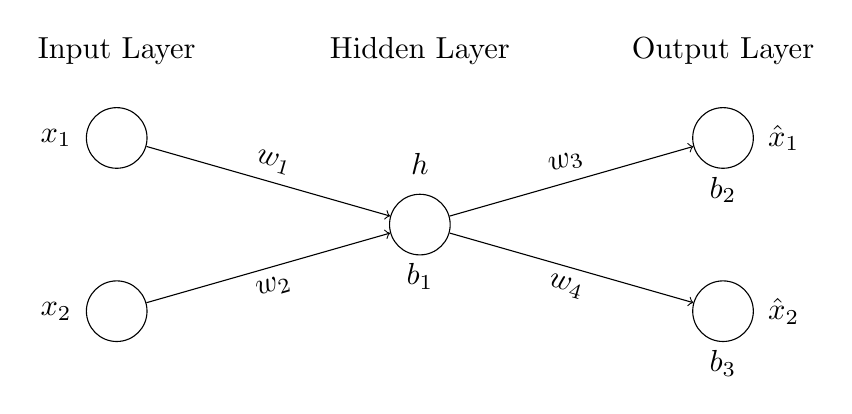
\begin{tikzpicture}[scale=1.1, transform shape]
% Input layer (2 neurons)
\node[circle, draw, minimum size=0.7cm] (input1) at (0, 1) {};
\node[circle, draw, minimum size=0.7cm] (input2) at (0, -1) {};
\node at (-0.7, 1) {$x_1$};
\node at (-0.7, -1) {$x_2$};
% Hidden layer (1 neuron)
\node[circle, draw, minimum size=0.7cm] (hidden) at (3.5, 0) {};
\node at (3.5, 0.7) {$h$};
% Output layer (2 neurons)
\node[circle, draw, minimum size=0.7cm] (output1) at (7, 1) {};
\node[circle, draw, minimum size=0.7cm] (output2) at (7, -1) {};
\node at (7.7, 1) {$\hat{x}_1$};
\node at (7.7, -1) {$\hat{x}_2$};
% Connections from input to hidden layer
\draw[->] (input1) -- node[above,sloped,pos=0.5] {$w_{1}$} (hidden);
\draw[->] (input2) -- node[below,sloped,pos=0.5] {$w_{2}$} (hidden);
% Connections from hidden layer to output
\draw[->] (hidden) -- node[above,sloped,pos=0.5] {$w_{3}$} (output1);
\draw[->] (hidden) -- node[below,sloped,pos=0.5] {$w_{4}$} (output2);
% Draw the labels for the layers
\node at (0, 2) {Input Layer};
\node at (3.5, 2) {Hidden Layer};
\node at (7, 2) {Output Layer};
% Biases
\node at (3.5, -0.6) {$b_1$};
\node at (7, 0.4) {$b_2$};
\node at (7, -1.6) {$b_3$};
\end{tikzpicture}
\end{center}
We can note that if we do indeed have a linear activation function, then the output of the hidden layer is given by: 
\begin{align*}
    E_\phi(\vec{x}) &= h = w_1 x_1 + w_2 x_2 + b_1 \\
\end{align*}
Similarly if we consider $h = E_\phi(x)$, then the output of the decoder is given by:
\begin{align*}
    D_\theta(h) &= \vec{\hat{x}} = \begin{bmatrix}
        w_3h + b_2 \\
        w_4h + b_3
    \end{bmatrix}
\end{align*}
Combining these two equations, we can see that the output of the autoencoder is given by:
\begin{align*}
    D_\theta(E_\phi(\begin{bmatrix}
        x_1 \\
        x_2
    \end{bmatrix})) &= \begin{bmatrix}
        w_3(w_1 x_1 + w_2 x_2 + b_1) + b_2 \\
        w_4(w_1 x_1 + w_2 x_2 + b_1) + b_3
    \end{bmatrix} \\
    &= \begin{bmatrix}
        w_3w_1 x_1 + w_3w_2 x_2 + w_3b_1 + b_2 \\
        w_4w_1 x_1 + w_4w_2 x_2 + w_4b_1 + b_3
    \end{bmatrix} \\
    &= \begin{bmatrix}
        w_1 w_3 & w_2 w_3\\
        w_1 w_4 & w_2 w_4
    \end{bmatrix} \begin{bmatrix}
        x_1 \\
        x_2
    \end{bmatrix} + \begin{bmatrix}
        w_3b_1 + b_2 \\
        w_4b_1 + b_3
    \end{bmatrix}
\end{align*}
We can see that with this architecture, a linear activation function, the autoencoder is essentially an affine linear transformation of the input data. 
We can also consider the MSE loss function in terms of this architecture. The MSE loss function is given by:
\begin{align*}
    L_{MSE}(\theta, \phi) &= \frac{1}{N} \sum_{i=1}^{N} |\vec{x}_i - D_\theta(E_\phi(\vec{x}_i))|^2 \\
    &= \frac{1}{N} \sum_{i=1}^{N} \left| \begin{bmatrix}
        x_{i,1} \\
        x_{i,2}
    \end{bmatrix} - \begin{bmatrix}
        w_1 w_3 & w_2 w_3\\
        w_1 w_4 & w_2 w_4
    \end{bmatrix} \begin{bmatrix}
        x_{i,1} \\
        x_{i,2}
    \end{bmatrix} - \begin{bmatrix}
        w_3b_1 + b_2 \\
        w_4b_1 + b_3
    \end{bmatrix} \right|^2 \\
    &= \frac{1}{N} \sum_{i=1}^{N} \left| \begin{bmatrix} 
        1 - w_1 w_3& -w_2 w_3\\
        -w_1 w_4 & 1 - w_2 w_4
    \end{bmatrix} \begin{bmatrix}
        x_{i,1} \\
        x_{i,2}
    \end{bmatrix} - \begin{bmatrix}
        w_3b_1 + b_2 \\
        w_4b_1 + b_3
    \end{bmatrix} \right|^2 \\
    &= \frac{1}{N} \sum_{i=1}^{N} \left| P X_i - Q \right|^2 
\end{align*}
For the sake of simplicity and ease of calculation early I will let $PX_i-Q = \vec{\ell}_i$ and $|PX_i-Q|^2$ as a constant $\alpha_i$.
\begin{align*}
    PX_i - Q &= \begin{bmatrix}
    (1-w_1 w_3)x_{i,1} - w_2 w_3 x_{i,2} - (w_3b_1 + b_2) \\
    -w_1 w_4 x_{i,1} + (1-w_2 w_4)x_{i,2} - (w_4b_1 + b_3)
    \end{bmatrix} &= \vec{\ell}_i\\
    |PX_i - Q|^2 &= \quad \text{Some atrocious calculation} &= \alpha_i
\end{align*}
Notice that is essentially the same as the loss function used in linear regression, where $P$ is the matrix of weights and $Q$ is the bias term. \\
We can consider the partial derivatives of the loss function with respect to the sets of parameters $\theta$ and $\phi$. For the sake of simplicity, we will only calculate the partial derivatives with respect to the $w_1, b_1$ and $w_3$ parameters.
\begin{align*}
    \frac{\partial L_{MSE}}{\partial w_1} &= \frac{\partial }{\partial w_1} \left( \frac{1}{N} \sum_{i=1}^{N} \left| P X - Q \right|^2 \right) \\
    &= \frac{1}{N} \sum_{i=1}^{N} 2 \left| P X - Q \right| \cdot \frac{\partial }{\partial w_1} \left| P X - Q \right| \quad \text{(Chain Rule)} \\
    &= \frac{1}{N} \sum_{i=1}^{N} - 2 \left| P X - Q \right| \cdot (w_3 x_1 + w_4 x_2) \\ 
    &= \frac{1}{N} \sum_{i=1}^{N} - 2 \sqrt{\alpha_i} \cdot (w_3 x_1 + w_4 x_2)
\end{align*}
\begin{align*}
    \frac{\partial L_{MSE}}{\partial b_1} &= \frac{\partial }{\partial b_1} \left( \frac{1}{N} \sum_{i=1}^{N} \left| P X - Q \right|^2 \right) \\
    &= \frac{1}{N} \sum_{i=1}^{N} 2 \left| P X - Q \right| \cdot \frac{\partial }{\partial b_1} \left| P X - Q \right| \quad \text{(Chain Rule)} \\
    &= \frac{1}{N} \sum_{i=1}^{N} - 2 \left| P X - Q \right| \cdot (w_3) \\
    &= \frac{1}{N} \sum_{i=1}^{N} - 2 \sqrt{\alpha_i} \cdot (w_3) 
\end{align*}
\begin{align*}
    \frac{\partial L_{MSE}}{\partial w_3} &= \frac{\partial }{\partial w_3} \left( \frac{1}{N} \sum_{i=1}^{N} \left| P X - Q \right|^2 \right) \\
    &= \frac{1}{N} \sum_{i=1}^{N} 2 \left| P X - Q \right| \cdot \frac{\partial }{\partial w_3} \left| P X - Q \right| \quad \text{(Chain Rule)} \\
    &= \frac{1}{N} \sum_{i=1}^{N} - 2 \left| P X - Q \right| \cdot (w_1 x_1 + w_2 x_2 - b_1) \\
    &= \frac{1}{N} \sum_{i=1}^{N} - 2 \sqrt{\alpha_i} \cdot (w_1 x_1 + w_2 x_2 - b_1)
\end{align*}
When we have more layers, more nodes, and more complex activation functions we can take the same approach as a regular neural network. If we want to minimize the loss function with respect to the parameters $\theta = (w_1, w_2, b_1)$ and $\phi = (w_3, w_4, b_2, b_3)$, we can use the chain rule to calculate the gradient of the loss function with respect to the parameters. The gradient of the loss function with respect to the $\theta$ parameters partials is given by:
\begin{align*}
    \frac{\partial L_{MSE}}{\partial w_1} &= \frac{\partial L_{MSE}}{\partial \hat{x}_1} \cdot \frac{\partial \hat{x}_1}{\partial h} \cdot \frac{\partial h}{\partial w_1} + \frac{\partial L_{MSE}}{\partial \hat{x}_2} \cdot \frac{\partial \hat{x}_2}{\partial h} \cdot \frac{\partial h}{\partial w_1} \\
    \frac{\partial L_{MSE}}{\partial w_2} &= \frac{\partial L_{MSE}}{\partial \hat{x}_1} \cdot \frac{\partial \hat{x}_1}{\partial h} \cdot \frac{\partial h}{\partial w_2} + \frac{\partial L_{MSE}}{\partial \hat{x}_2} \cdot \frac{\partial \hat{x}_2}{\partial h} \cdot \frac{\partial h}{\partial w_2} \\
    \frac{\partial L_{MSE}}{\partial b_1} &= \frac{\partial L_{MSE}}{\partial \hat{x}_1} \cdot \frac{\partial \hat{x}_1}{\partial h} \cdot \frac{\partial h}{\partial b_1} + \frac{\partial L_{MSE}}{\partial \hat{x}_2} \cdot \frac{\partial \hat{x}_2}{\partial h} \cdot \frac{\partial h}{\partial b_1} \\
\end{align*}
And the $\phi$ parameters partials are given by:
\begin{align*}
    \frac{\partial L_{MSE}}{\partial w_3} &= \frac{\partial L_{MSE}}{\partial \hat{x}_1} \cdot \frac{\partial \hat{x}_1}{\partial w_3} + \frac{\partial L_{MSE}}{\partial \hat{x}_2} \cdot \frac{\partial \hat{x}_2}{\partial w_3} \\
    \frac{\partial L_{MSE}}{\partial w_4} &= \frac{\partial L_{MSE}}{\partial \hat{x}_1} \cdot \frac{\partial \hat{x}_1}{\partial w_4} + \frac{\partial L_{MSE}}{\partial \hat{x}_2} \cdot \frac{\partial \hat{x}_2}{\partial w_4} \\
    \frac{\partial L_{MSE}}{\partial b_2} &= \frac{\partial L_{MSE}}{\partial \hat{x}_1} \cdot \frac{\partial \hat{x}_1}{\partial b_2} + \frac{\partial L_{MSE}}{\partial \hat{x}_2} \cdot \frac{\partial \hat{x}_2}{\partial b_2} \\
    \frac{\partial L_{MSE}}{\partial b_3} &= \frac{\partial L_{MSE}}{\partial \hat{x}_1} \cdot \frac{\partial \hat{x}_1}{\partial b_3} + \frac{\partial L_{MSE}}{\partial \hat{x}_2} \cdot \frac{\partial \hat{x}_2}{\partial b_3}
\end{align*}
We can consider the terms of $w_1$ and compute out the partials similar to the previous example.
\begin{align*}
    \frac{\partial L_{MSE}}{\partial w_1} &= \frac{\partial L_{MSE}}{\partial \hat{x}_1} \cdot \frac{\partial \hat{x}_1}{\partial h} \cdot \frac{\partial h}{\partial w_1} + \frac{\partial L_{MSE}}{\partial \hat{x}_2} \cdot \frac{\partial \hat{x}_2}{\partial h} \cdot \frac{\partial h}{\partial w_1} \\
    \frac{\partial L_{MSE}}{\partial \hat{x}_1} &= \frac{1}{N} \sum_{i=1}^{N} - 2 \left| \begin{bmatrix}
        x_1 \\
        x_2
    \end{bmatrix} - \begin{bmatrix}
        \hat{x}_1 \\
        \hat{x}_2
    \end{bmatrix} \right|\\
    \frac{\partial \hat{x}_1}{\partial h} &= \frac{\partial }{\partial h} \left( w_3h + b_2 \right) = w_3\\
    \frac{\partial h}{\partial w_1} &= \frac{\partial }{\partial w_1} \left( w_1 x_1 + w_2 x_2 + b_1 \right) = x_1\\
    \frac{\partial L_{MSE}}{\partial \hat{x}_2} &= \frac{1}{N} \sum_{i=1}^{N} - 2 \left| \begin{bmatrix}
        x_1 \\
        x_2
    \end{bmatrix} - \begin{bmatrix}
        \hat{x}_1 \\
        \hat{x}_2
    \end{bmatrix} \right|\\
    \frac{\partial \hat{x}_2}{\partial h} &= \frac{\partial }{\partial h} \left( w_4h + b_3 \right) = w_4\\
    \frac{\partial h}{\partial w_1} &= \frac{\partial }{\partial w_1} \left( w_1 x_1 + w_2 x_2 + b_1 \right) = x_2\\
    \frac{\partial L_{MSE}}{\partial w_1} &= \frac{1}{N} \sum_{i=1}^{N} - 2 \left| \begin{bmatrix}
        x_1 \\
        x_2
    \end{bmatrix} - \begin{bmatrix}
        \hat{x}_1 \\
        \hat{x}_2
    \end{bmatrix} \right| \cdot \left( w_3 x_1 + w_4 x_2 \right)\\
    &- \frac{1}{N} \sum_{i=1}^{N} - 2 \left| \sqrt{\alpha_i} \right| \cdot \left( w_3 x_2 + w_4 x_1 \right)\\
\end{align*}
We can see that (obviously) the partial derivative of the loss function, both from the matrix perspective and the neural network perspective, is the same. 

\section{Conclusion}
Both PCA and Autoencoders are great methods for dimensionality reduction. And though they are different methods, they are closely related. Their main similaries lie in the fact that they both aim to find the best lower dimensional representation of the data. PCA does this by finding the directions of maximum variance, while autoencoders do this by learning a non-linear mapping from the input data to a lower-dimensional representation. The main difference between the two methods, as we can see above, is the method of training. For PCA, we use the covariance matrix to find the directions of maximum variance, which means we need the entire dataset immediately, which has issues with large datasets. On the other hand, autoencoders can be trained in an online fashion, meaning we can train them on small batches of data at a time. But this means we need time to train the autoencoder for it to converge to the optimal solution.\\
I do not have time but I will be working on it beyond this assignment to see how long for convergence for this linear autoencoder to the PCA solution. 
\end{document}